\documentclass{article}

\usepackage[cm]{fullpage}
\usepackage[russian]{babel}
\usepackage{amssymb}
\usepackage{amsmath}
\usepackage{setspace}
\usepackage{titlesec}
\usepackage{mdframed}
\usepackage{xcolor}
\usepackage{graphicx}
\usepackage{subcaption}
\usepackage{indentfirst}
\usepackage{titlesec}
\usepackage{accents}
\usepackage{hyperref}

\usepackage{float}

% Headers
\titleformat{\section}{\normalfont \Large \bfseries}{\thesection .}{0.2cm}{}
\titlespacing{\section}{0pt}{*-1}{*-1}

\titleformat{\subsection}{\normalfont \large \bfseries}{\thesubsection .}{0.2cm}{}
\titlespacing{\subsection}{3pt}{*-1}{*-2}

\titleformat{\subsubsection}{\normalfont \bfseries}{\thesubsubsection .}{0.2cm}{}
\titlespacing{\subsubsection}{6pt}{*-1}{*-2}

% Space between rows
\linespread{1.5}

% Space between paragraphs
\setlength{\parindent}{1cm}
\setlength{\parskip}{0.5cm}

% Commands
\newcommand{\R}{\mathbb R}
\newcommand{\E}[1]{\textsf E \left[ #1 \right]}
\newcommand{\Var}[1]{\textsf{Var} \left( #1 \right)}
\newcommand{\intR}{\int_{\R}}
\newcommand{\arc}[1]{\accentset{\smallsmile}{#1}}

% Operators


\begin{document}

\section{ВВЕДЕНИЕ}

\section{ТЕОРЕТИЧЕСКОЕ ОПИСАНИЕ МОДЕЛИ}

Рассмотрим модель
\[
d S_t = f \left( M_t \right) dt + \sigma_t d W_t \quad \overset{def}{\Leftrightarrow} \quad S_t = \int\limits_0^t f \big( M_s \big) ds + \int\limits_0^t \sigma_s d W_s, \quad (1)
\]
где $S_t$ - логарифм зависимой переменной, $f$ - некоторая функция от $M_t$ - матрицы ''объекты-признаки'', $\sigma_t$ - параметр, в общем случае непостоянный, $W_t$ - броуновское движение.

Заметим, что выражение $(1)$ можно представить в виде
\[
S_{k \Delta} - S_{(k - 1) \Delta} = \left( f \big( M_{k \Delta}  \big) - f \big( M_{(k - 1) \Delta} \big) \right) \Delta + \sigma_{k \Delta} \left(W_{k \Delta} - W_{(k - 1) \Delta} \right), \quad (2)
\]
где $k \Delta$ и $(k - 1) \Delta$ - некоторые моменты времени на сетке $\{\Delta, 2 \Delta, ... , n \Delta\}$. Тогда, деление обеих частей $(2)$ на $\sqrt{\Delta}$ даст
\[
\frac{ S_{k \Delta} - S_{(k - 1) \Delta}}{\sqrt{\Delta}} = \left( f \big( M_{k \Delta} \big) - f \big( M_{(k - 1) \Delta} \big) \right) \sqrt{\Delta} +  \sigma_{k \Delta} \frac{\left( W_{k \Delta} - W_{(k - 1) \Delta} \right)}{\sqrt{\Delta}}. \quad (3)
\]

Также известно, что $ W_{k \Delta} - W_{(k - 1) \Delta} \sim \mathrm{N} (0, \Delta).$ Следовательно,  $\frac{W_{k \Delta} - W_{(k - 1) \Delta}}{\sqrt{\Delta}} \sim \mathrm{N}(0, 1)$.

Поэтому
\[
\frac{ S_{k \Delta} - S_{(k - 1) \Delta}}{\sqrt{\Delta}} = \left( f \big( M_{k \Delta} \big) - f \big( M_{(k - 1) \Delta} \big) \right) \sqrt{\Delta} +  \sigma_{k \Delta} Z_{k \Delta}, \quad Z_{k \Delta} \sim \mathcal{N}(0, 1). \quad (4)
\]

\section{РЕКУРРЕНТНЫЕ НЕЙРОННЫЕ СЕТИ}

\subsection{Базовая RNN}

Для обработки последовательных данных зачастую используют рекуррентные нейронные сети (далее RNN - recurrent neural networks). Их ключевой особенностью является использование при обучении предшествующих данных наряду с текущими, что схематично представлено на Рис. 1.

\begin{figure}[H]
    \centering
    \includegraphics[width=0.5\textwidth]{/Users/mmenadzhiev/Desktop/Studying/Project/Estimation of the price/Отчет/Images/rnn.png}
    \caption{Структура простейшей RNN}
\end{figure}

В общих чертах принцип работы простейшей RNN подразумевает сохранение результатов обучения на предыдущих относительно текущего значениях и их использования для более качественного прогнозирования. Действительно, в контексте временных редов и последовательных данных в целом история очевидно играет значительную роль, поэтому такой подход является вполне разумным.

При этом базовая структура RNN может повлечь несколько значительных проблем при обучении, например, таких как \textbf{взрыв} или \textbf{затухание градиентов} (vanishing or exploding gradients). Проще всего ее осознать на конкретном примере. Так, на Рис. 2 представлен частный случай RNN, в котором за передачу информации от предыдущего значения к текущему отвечает параметр $W_2$. Также понятно, что при обратном проходе по графу (поиске производных по параметрам) в цепочке произведения частных производных мы так или иначе получим $W_2^2$. Следовательно, при числе слоев $n$ мы столкнемся с множителем $W_2^n$, и тогда если $|W_2| < 1$, то $W_2^n \to 0$ при $n \to \infty$, что называется затуханием градиента. Аналогично при $|W_2| > 1 \; W_2^n \to \infty$ при $n \to \infty$ - взрыв градиента.

\begin{figure}[H]
    \centering
    \includegraphics[width=0.5\textwidth]{/Users/mmenadzhiev/Desktop/Studying/Project/Estimation of the price/Отчет/Images/rnn2.png}
    \caption{Частный пример RNN $\text{}^1$}
\end{figure}

Заметим, что выявленные проблемы действительно значительны, так как при затухании градиента веса фактически перестают обновляться, а при взрыве - наоборот меняются слишком сильно и препятствуют нахождению оптимума, что следует из формулы
\[
w_t = w_{t - 1} - \frac 1 \eta Q(w_{t - 1}), \quad (5)
\]
где $w_t$ - вектор весов в момент $t$, $\eta$ - скорость обучения, $Q(x)$ - градиент функции потерь.

Таким образом, для решения нашей задачи необходимо более продуманная реализация RNN, не имеющая вышеописанных недостатков, например, LSTM (Long Short-Term Memory), которую мы рассмотрим в дальнейшем.

\subsection{Long Short-Term Memory}

Перейдем к описанию следующего поколения RNN - модели LSTM (Long Short-Term Memory). Данная модификация простейшей рекуррентной нейронной сети позволяет избежать такой значительной проблемы, как затухание или взрыв градиента засчет специальной структуры, схематично представленной на Рис. 3.

\begin{figure}[H]
    \centering
    \includegraphics[width=0.5\textwidth]{/Users/mmenadzhiev/Desktop/Studying/Project/Estimation of the price/Отчет/Images/LSTM.png}
    \caption{Структура LSTM}
\end{figure}

Основная идея LSTM-сетей заключается в использовании двух потоков информации, влияющих на конечный прогноз напрямую - краткосрочной и долгосрочной памяти (Рис. 4). Заметим, что в базовой RNN  долгосрочные данные имели лишь опосредованное значение через последовательное суммирование и применение функций активации (Рис. 2).

\begin{figure}[H]
    \centering
    \includegraphics[width=0.3\textwidth]{/Users/mmenadzhiev/Desktop/Studying/Project/Estimation of the price/Отчет/Images/LSTM2.png}
    \caption{Иллюстрация влияния долгосрочной и краткосрочной памяти в рамках LSTM-модели$\text{}^2$}
\end{figure}

Наконец перейдем к более подробному описанию LSTM. Для начала еще раз обратимся к Рис. 3, на котором видно, что в рамках данной модели используются две функции активации - сигмоида ($\sigma$) и гиперболический тангенс ($tanh$). Вспомним, как они задаются
\begin{enumerate}
\item Сигмоида:
\[
\sigma(x) = \frac{e^x}{1 + e^x}, \quad (6)
\]
причем $\sigma: \mathbb R \mapsto (0, 1)$.

\item Гиперболический тангенс:
\[
tanh(x) = \frac{e^x - e^{-x}}{e^x + e^{-x}}, \quad (7)
\]
причем $tanh: \mathbb R \mapsto (-1, 1)$.
\end{enumerate}

Что касается одной составляющей LSTM-модели, то ее условно можно разделить на три блока, представленных на Рис. 5, в котором розовой линией обозначена краткосрочная память, а зеленой - долгосрочная. Также функция в маленьком голубом прямоугольнике есть сигмоида, а в маленьком оранжевом - гиперболический тангенс.

Первый блок выделен большим голубым прямоугольником, в котором по существу происходит определение доли от входящего значения \textit{долгосрочной} памяти, которую необходимо оставить для дальнейшего использования.

Второй блок образован большим зеленым и большим оранжевым прямоугольниками. В большом оранжевом прямоугольнике вычисляется потенциальная \textit{долгосрочная} память, а в синем - аналогично первому блоку доля, которую модель запомнит. Затем найденное значение будет сложено с получившимся после первого блока, что образует новую \textit{долгосрочную} память, которая будем передана в дальнейшие итерации модели.

Третий блок получается из объединения большого фиолетого и большого розового прямоугольников. В нем и образуется выход, который либо передается в последующие части модели, аналогичные текущей, в качестве новой \textit{краткосрочной} памяти, либо уже представляет конечный результат. Более конкретно, в третьем блоке на основе новой \textit{долгосрочной} памяти определяется потенциальная \textit{краткосрочная}, и по известной схеме из первого блока определяется ее доля.

\begin{figure}[H]
    \centering
    \includegraphics[width=0.5\textwidth]{/Users/mmenadzhiev/Desktop/Studying/Project/Estimation of the price/Отчет/Images/LSTM3.jpg}
    \caption{Частный пример LSTM$\text{}^2$}
\end{figure}

Заметим, что для получения произвольного прогноза, например, в задаче регрессии, можно к выходу модели добавить полносвязный слой. Таким образом, LSTM является универсальной нейросетью, позволяющей работать с последовательной информацией, что актуально и для нашей задачи.

\section{ОЦЕНКА ФУНКЦИИ $f$}

\subsection{Описание компонент модели и подхода к оцениванию}

Для начала вспомним, как выглядит наша модель согласно уравнению (4)
\[
\frac{ S_{k \Delta} - S_{(k - 1) \Delta}}{\sqrt{\Delta}} = \left( f \big( M_{k \Delta} \big) - f \big( M_{(k - 1) \Delta} \big) \right) \sqrt{\Delta} +  \sigma_{k \Delta} Z_{k \Delta}, \quad Z_{k \Delta} \sim \mathcal{N}(0, 1),
\]
где $f$ - некоторая функция от $M_t$ - матрицы ''объекты-признаки'', в которой находятся некоторые временные показатели, соответствующие зависимой переменной, например, лаги порядка от 1 до $h, \, h \in \mathbb N$. Иными словами, строки матрицы $M_t$ состоят из последовательностей временных данных, для обработки которых, как уже было описано выше, возможно использование рекуррентных нейронных сетей, и в частности LSTM-модели, которую мы и будем обучать для оценки функции $f$.

Также в данном разделе предположим постоянство $\sigma$, то есть $\sigma_{\Delta k} = \sigma, \, \forall k = 0, 1, ... $. Следовательно, текущая модель выглядит как
\[
\frac{ S_{k \Delta} - S_{(k - 1) \Delta}}{\sqrt{\Delta}} = \left( f \big( M_{k \Delta} \big) - f \big( M_{(k - 1) \Delta} \big) \right) \sqrt{\Delta} +  \sigma Z_{k \Delta}, \quad Z_{k \Delta} \sim \mathcal{N}(0, 1). \quad (8)
\]

Теперь более подробно рассмотрим матрицу $M_t$. В базовом варианте она содержит исключительно лаги некоторой объясняющей переменной, коррелирующей с зависимой. Для более подробного объяснения обратимся к примеру. Пусть $y_t$ - зависимая переменная, в нашем случае $y_t = \frac{S_t - S_{t - 1}}{\sqrt{\Delta}}$, а $x_t$ - объясняющая переменная, связь которой с $y_t$ чем-либо обоснована. Тогда если $h, \, h \in \mathbb N$ - максимальный порядок лага, то матрица ''объекты-признаки'' на момент $t$ есть
\[
M_t = \begin{bmatrix}
    x_{1} & x_{2} & \cdots & x_{h} \\
    x_{2} & x_{3} & \cdots & x_{h + 1} \\
    \vdots & \vdots & \ddots & \vdots \\
    x_{t - h} & x_{t - h + 1} & \cdots & x_{t - 1} 
\end{bmatrix}_.
\]

В большинстве случаев модели машинного обучения обладают \textit{гиперпараметрами} - параметрами, не участвующими в обучении, значения которых необходимо выбрать заранее на основе каких-либо принципов, например, кросс-валидации. Что касается рассматриваемой модели, соответствующей уравнению (8), то ее \textit{гиперпараметры} есть:

\vspace{-20pt}

\begin{itemize}

\item $\sigma$ - параметр, отвечающий за волатильность

\item $\Delta$ - размерность временной сетки

\item $h$ - количество лагов объясняющей переменной, используемое при оценке

\end{itemize}

\vspace{-10pt}

Наконец определим функцию потерь, при помощи которой будет происходить оценка функции $f$. Заметим, что в таблице $M_{k - 1} \Delta$ находится лаг порядка $h$, а минимальный допустимый номер наблюдения есть 1. Следовательно, наименьший доступный $k$ равен $h + 2$. Тогда функцию потерь можно записать как
\[
L = \sum\limits_{k = h + 2}^n \left( \frac{S_{k \Delta} - S_{(k - 1) \Delta}}{\sqrt{\Delta}} - \left( f(M_{k \Delta}) - f(M_{(k - 1) \Delta}) \right) \sqrt{\Delta} - \sigma Z_{k \Delta} \right)^2, \quad (9).
\]

\subsection{Выбранные данные}

В качестве конкретных примеров я решил взять зависимость цены криптовалюты Ethereum (ETH) от цены криптовалюты Bitcoin (BTC). Данный выбор обосновывается существенной взаимосвязью данных временных рядов, что подтверждается значением корреляции, равным 0.934 на выбранных данных, а также визуальным сходством, представленным на Рис. 6.

\begin{figure}[H]
    \centering
    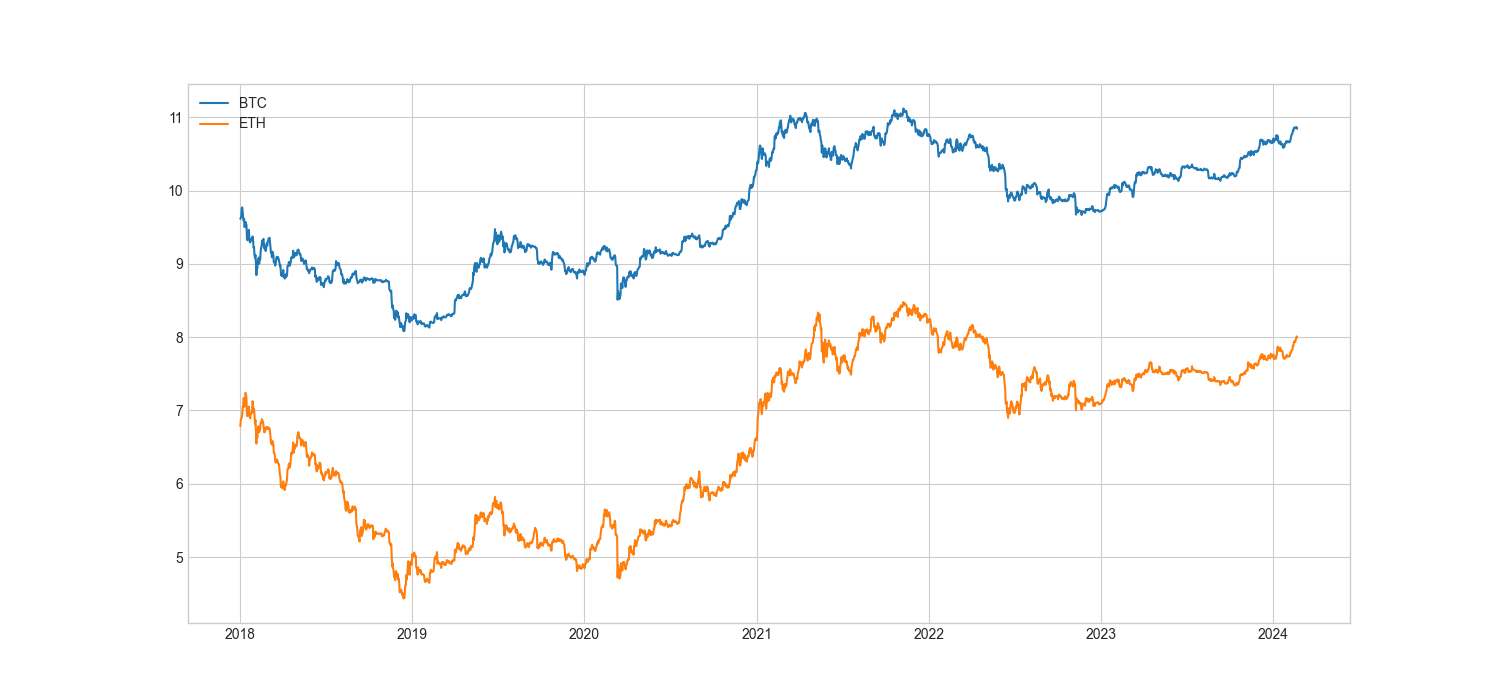
\includegraphics[width=\textwidth]{/Users/mmenadzhiev/Desktop/Studying/Project/Estimation of the price/Final code/Images/log_btc_eth.png}
    \caption{Динамики логарифмов цен BTC и ETH}
\end{figure}

\subsection{Одношаговое прогнозирование}

Для начала определим \textit{одношаговое} прогнозирование как следующий процесс:

\vspace{-15pt}

\begin{enumerate}
\item Фиксируются \textit{тренировочная} и \textit{тестовая} выборки

\item Модель единожды обучается на \textit{тренировчной} выборке

\item Строится прогноз на \textit{тестовую} выборку

\item Оценивается результативность модели
\end{enumerate}

\vspace{-15pt}

Иными словами, \textit{одношаговое} прогнозирование совпадает с базовым подходом к прогнозированию в машинном обучении.

Также мы будем использовать $\Delta = 1$, поэтому необходимо подобрать только гиперпараметры $h$ и $\sigma$. Для этого воспользуемся \textit{кросс-валидацией} по набору параметров
\[
h \in \{ 5, 10, 20, 50, 100, 200 \}, \quad \sigma \in \{ 0, 0.001, 0.01, 0.03, 0.05 \},
\]
то есть переберем все возможные пары и выберем ту, при которой модель выдаст наилучший результат. При этом размер тестовой выборки составит 50 наблюдений.

Сначала посмотрим на поведение модели на тестовых данных при фиксированном параметре $h$, равном 20, и различных $\sigma \in \{ 0, 0.001, 0.01, 0.03, 0.05 \}$  (Рис. 7). По графикам видно, что с ростом $\sigma$ волатильность приращения логарифма цен также увеличивается, из чего можно сделать вывод о значимости данного параметра.

\begin{figure}[H]
    \centering
    \includegraphics[width=\textwidth]{/Users/mmenadzhiev/Desktop/Studying/Project/Estimation of the price/Final code/Images/one_step_h=20.png}
    \caption{Предсказания модели на тестовой выборке при фиксированном $h = 20$}
\end{figure}

Теперь зафиксируем $\sigma = 0.01$ и посмотрим на то, как предсказания зависят от количества используемых лагов $h$ (Рис. 8). Легко видеть, что результаты фактически остаются постоянными, что говорит о том, что увеличение числа учитываемых лагов не влияет значительно на получаемый результат. С точки зрения интуиции это может означать то, что на приращение логарифма цен влияет только ближайшая известная информация. Действительно, как правило изменения цен являются реакцией на некоторые события и зачастую происходят практически мгновенно. Поэтому весьма разумно допустить, что чем больше времени прошло с момента события, тем слабее его влияение на показатель в рассматриваемый период.

\begin{figure}[H]
    \centering
    \includegraphics[width=\textwidth]{/Users/mmenadzhiev/Desktop/Studying/Project/Estimation of the price/Final code/Images/one_step_sigma=0.01.png}
    \caption{Предсказания модели на тестовой выборке при фиксированной $\sigma = 0.01$}
\end{figure}

Таким образом, стоит сделать одно важное наблюдение относительно различий в прогнозировании \textit{несезонного} показателя как такового, в нашем случае логарифма цены, и в прогнозировании его приращений. Сразу отметим, что \textit{несезонность} гарантирует отсутствие устойчивой связи между периодами спустя длинные промежутки времени, что важно для дальнейшего рассуждения. Итак, прогнозирование приращений такого показателя позволяет избежать использования большого объема данных, так как требует лишь информации о ближайших периодах, тогда как в абсолютном значении может быть заложены более фундаментальные факторы, имеющие свое начало из относительно давних событий. Следовательно, предсказывание приращений потенциально является более предпочтительным.

\subsection{Многошаговое прогнозирование}

В отличие от \textit{одношагового} прогнозирования \textit{многошаговое} строится следующим образом:

\vspace{-15pt}

\begin{enumerate}
    
    \item

\end{enumerate}


\section{Источники}

[1] StatQuest with Josh Starmer: \href{https://youtu.be/AsNTP8Kwu80?si=N-Snml3hPPGoP0i3}{Recurrent Neural Networks (RNNs)}

[2] StatQuest with Josh Starmer: \href{https://www.youtube.com/watch?v=YCzL96nL7j0&list=PLblh5JKOoLUIxGDQs4LFFD--41Vzf-ME1&index=16&ab_channel=StatQuestwithJoshStarmer}{Long Short-Term Memory (LSTM)}

\end{document}
